\section*{Definición de Función}

%- - - - - - - - - - - - - - - - - Título - - - - - - - - - - - - - - - - - -%
\begin{frame}[c] 
\centering
\huge \textbf{Definición de Funcion}
\end{frame}



% - - - - - - - - - - - - - - - - - Slide 01 - - - - - - - - - - - - - - - -
\begin{frame}
    \frametitle{Definición de Funcion}
    \justify
    \hspace{5mm}Un problema difícil es más sencillo al dividirlo en pequeñas partes y tratar de buscar la solución de cada una de ellas y así resolver todo el problema general, la mejor forma de elaborar
    y dar mantenimiento a un programa complejo es construirlo a partir de bloques menores o módulos.\\
    \hspace{5mm}Dichos módulos se escriben solamente una vez, pero pueden ser llamados en diferentes puntos del programa principal o de cualquier otro módulo.
\end{frame}


% - - - - - - - - - - - - - - - - - Slide 02 - - - - - - - - - - - - - - - -
\begin{frame}
\frametitle{Definición de Funcion}
\justify
\hspace{5mm}En lenguaje C a cada módulo o subprograma se le conoce como función; en este lenguaje se trabaja a base de funciones y, de manera general, los programas se elaboran combinando funciones que el programador escribe y funciones “predefinidas” disponibles en la biblioteca estándar de C.
\begin{center}
    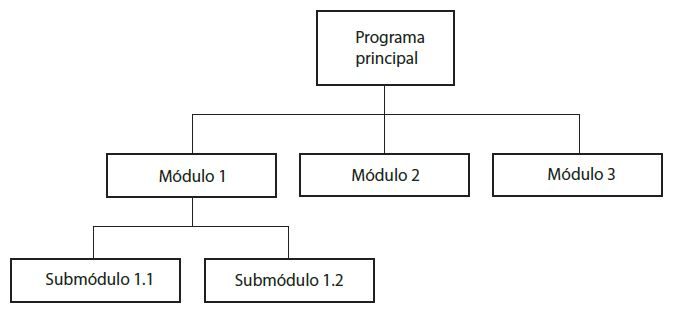
\includegraphics[scale=0.4]{figs/diagramaProgramacionModular.jpg}
\end{center}
\end{frame}



% - - - - - - - - - - - - - - - - - Slide 03 - - - - - - - - - - - - - - - -
\begin{frame}
    \frametitle{Definición de Funcion}
    \begin{center}
        \textbf{Ventajas de la programación modular}
    \end{center}
    \vspace{-8mm}
    \begin{itemize}
        \item Facilita el diseño descendente \textit{(proceso mediante el cual un problema se descompone en un serie de niveles o pasos sucesivos)}.\pause
        \item Se simplifica un algoritmo complejo.\pause
        \item Cada módulo se puede elaborar de manera independiente, lo que permite trabajar simultáneamente a varios programadores y disminuir el tiempo de elaboración del algoritmo.\pause
        \item La depuración se lleva a cabo en cada módulo.\pause
        \item El mantenimiento es más sencillo.\pause
        \item Creación de bibliotecas con módulos específicos (se pueden utilizar en otros programas).
    \end{itemize}
\end{frame}



% - - - - - - - - - - - - - - - - - Slide 04 - - - - - - - - - - - - - - - -
\begin{frame}
\frametitle{Definición de Funcion}
\begin{center}
    \textbf{Función}
\end{center}
\hspace{5mm}Es un subprograma que realiza una tarea específica que puede o no recibir valores (parámetros). En C podemos devolver cualquier tipo de datos escalares tipo numérico y el tipo carácter o en su caso regresar un valor nulo que llamaremos nada o ninguno). El uso de funciones es una práctica común y recomendable ya que permite dividir el código, simplificando así el desarrollo y la depuración del mismo.
\end{frame}